\documentclass{beamer}
%
% Choose how your presentation looks.
%
% For more themes, color themes and font themes, see:
% http://deic.uab.es/~iblanes/beamer_gallery/index_by_theme.html
%
\mode<presentation>
{
  \usetheme{default}      % or try Darmstadt, Madrid, Warsaw, ...
  \usecolortheme{crane} % or try albatross, beaver, crane, ...
  \usefonttheme{structurebold}  % or try serif, structurebold, ...
  \setbeamertemplate{navigation symbols}{}
  \setbeamertemplate{caption}[numbered]
} 

\usepackage[english]{babel}
\usepackage[utf8x]{inputenc}

\usepackage{listings}

\title[ML]{Machine Learning}
\author{Pawel Wocjan}
\institute{University of Central Florida}
\date{Spring 2019}

\begin{document}

\begin{frame}
  \titlepage
\end{frame}

% Uncomment these lines for an automatically generated outline.
%\begin{frame}{Outline}
%  \tableofcontents
%\end{frame}

\begin{frame}{Layers: the building blocks of deep learning}
\begin{itemize}
\item The fundamental data structure in neural networks is the {\bf layer}.
\item A layer is a data-processing module that takes as input one or more tensors and that outputs one or more tensors.
\item Some layers are stateless, but more frequently layers have a state: the layers {\bf weights}, one or several tensors learned with stochastic gradient descent, which together contain the network's {\bf knowledge}.
\end{itemize}
\end{frame}

\begin{frame}{Layers: the building blocks of deep learning}
\begin{itemize}
\item Different layers are appropriate for different tensor formats and different types of data processing.
\item Simple vector data, stored in 2D tensors of shape \texttt{(samples, features)} is often processed by {\bf densely connected layers}, also called {\bf fully connected layers} (the \texttt{Dense} class in Keras).
\item Sequence data, stored in 3D tensors of shape \texttt{(samples, timesteps, features)}, is typically processed by {\bf recurrent} layers such as {\bf long-short term memory (LSTM)} layer.
\item Image data, stored in 4D tensors, is usually processed by 2D \textbf{convolutional} layers (\texttt{Con2D}). 
\end{itemize}

\url{https://keras.io/layers/core/}

\url{https://keras.io/layers/convolutional/}

\url{https://keras.io/layers/recurrent/}
\end{frame}

\begin{frame}{Layers: the building blocks of deep learning}

\begin{itemize}
\item You can think of layers as LEGO bricks of deep learning.
\item Building deep-learning models in Keras is done by combining compatible layers to form useful data-processing pipelines.
\item Layer compatibility means that every layer will only accept input tensors of a certain shape and will return output tensors of a certain shape.
\item When using Keras, you don't have to worry about compatibility, because the layers you add to your model are dynamically built to match the shape of the incoming layer.
\end{itemize}
\end{frame}

\begin{frame}[fragile]{Layers: the building blocks of deep learning}
\lstset{language=Python,basicstyle={\small\ttfamily}}
\begin{lstlisting}
from keras import models
from keras import layers

network = models.Sequential()

network.add(layers.Dense(512,
                         activation='relu',
                         input_shape=(28 * 28,)))

# no need to specify input_shape for second layer
network.add(layers.Dense(10,
                         activation='softmax')) 
\end{lstlisting}
The second layer didn't receive an input shape argument -- instead, it automatically inferred its input shape as being the output shape of the first layer.
\end{frame}

\begin{frame}{Models: networks of layers}
\begin{itemize}
\item A deep-learning model is a directed, acyclic graph of layers. 
\item The most common topology is a linear stack of layers, mapping a single input to a single output. These can be implemented using \texttt{models.Sequential()}.
\item Initially, we will only work with linear stacks of layers. 
\item Later, we will also look at other network topologies such as two-branch networks, multi-head networks, and inception blocks.
\end{itemize}
{\small \url{https://keras.io/getting-started/sequential-model-guide/}}
\end{frame}

\begin{frame}{Models: networks of layers}
\begin{itemize}
\item The topology of a network defines a \textbf{hypothesis space}. 
\item By choosing a network topology, you constrain your \textbf{space of possibilities} (hypothesis space) to a specific series of tensor operations, mapping input data to output data.
\item You'll be then searching for a good set of values for the weight tensor involved in these tensor operations using stochastic a variant of gradient descent.
\item Picking the right network architecture is more art than a science. We will study explicit principles for building neural networks and develop intuition as to what works or doesn't for specific problems.
\end{itemize}
\end{frame}


\begin{frame}{Loss functions \& optimizers: keys to configuring the learning process}
\begin{itemize}
\item Once the network architecture is defined, you still need to do two things:
\begin{itemize}

\medskip
\item \textbf{Loss function (objective function)}

The quantity that will be minimized during training. It represents a measure of success for that task at hand.

\url{https://keras.io/losses/}

\medskip
\item \textbf{Optimizer} Determines how the network will be updated based on the loss function. Implements a specific variant of stochastic gradient descent (SGD).

\url{https://keras.io/optimizers/}
\end{itemize}
\end{itemize}
\end{frame}


\begin{frame}{Loss functions \& optimizers: keys to configuring the learning process}
\begin{itemize}
\item Choosing the right objective function for the right problem is extremely important: your network will take any shortcut it can, to minimize the loss.
\item Fortunately, there are simple guidelines you can use to choose the correct loss for common problems such as classification, regression, and sequence prediction.
\end{itemize}
{\footnotesize
\begin{tabular}{|c|c|c|}
\hline
Problem type & Last-layer activation & Loss function \\ \hline\hline
Binary classification & \texttt{sigmoid} & \texttt{binary\_crossentropy} \\ \hline
Multiclass,  & \texttt{softmax} & \texttt{categorical\_crossentropy} \\
single-label classification & & \\ \hline
Multiclass,  & \texttt{sigmoid} & \texttt{binary\_crossentropy} \\
multi-label classification & & \\ \hline
Regression & \texttt{None} & \texttt{mse} \\
to arbitrary values & & \\ \hline
Regression & \texttt{sigmoid} & \texttt{mse} or \\
to values in $[0,1]$ & & \texttt{binary\_crossentropy} \\ \hline
\end{tabular}
}
\end{frame}

\end{document}

%%%%%%%%%%%%%%%%%%%%%%%%%%%%%%%%%%%%%%%%%%%%%%%

\begin{frame}{}
\begin{itemize}
\item 
\end{itemize}
\end{frame}

\begin{frame}{}
\begin{itemize}
\item 
\end{itemize}
\end{frame}

%%%%%%%%%%%%%%%%%%%%%%%%%%%%%%%%%%%%%%%%%%%%%%%

\begin{frame}{Sources for Slides}

\begin{itemize}
\item I have extensively used the machine learning materials that have been prepared by Google. 

\medskip
\footnotesize{ 
\url{https://developers.google.com/machine-learning/crash-course/}
}

\item Google has licensed these materials under the Creative Commons Attribution 3.0 License.

\medskip
\footnotesize{ 
\url{https://creativecommons.org/licenses/by/3.0/}
}
\end{itemize}
\end{frame}

\begin{frame}{TensorFlow}
\begin{itemize}
    \item TensorFlow is a computational framework for building machine learning models. 
    \item TensorFlow provides a variety of different toolkits that allow you to construct models at your preferred level of abstraction. 
    \item You can use lower-level APIs to build models by defining a series of mathematical operations. 
    \item Alternatively, you can use higher-level APIs (like \texttt{tf.estimator}) to specify predefined architectures, such as linear regressors or neural networks.
    \item 
\end{itemize}
\end{frame}

\begin{frame}{TensorFlow}
\begin{itemize}
    \item The following figure shows the current hierarchy of TensorFlow toolkits:
\end{itemize}

\medskip
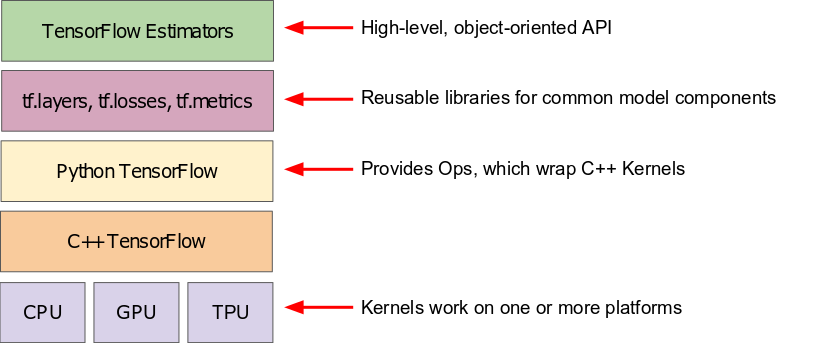
\includegraphics[width=1.0\textwidth]{images/TFHierarchy.png}
\end{frame}

\begin{frame}{TensorFlow}
\begin{itemize}
    \item The following table summarizes the purposes of the different layers:
\end{itemize}

\medskip
\begin{tabular}{|l|l|}
    \hline
    Toolkit(s) & Description \\ \hline \hline
    Estimator \texttt{tf.estimator} & High-level, OOP API \\ \hline
    \texttt{tf.layers/tf.losses/} & Libraries for common model \\
    \texttt{tf.metrics}           & components \\ \hline
    TensorFlow & Lower-level APIs \\ \hline
\end{tabular}
\end{frame}


\begin{frame}{TensorFlow}
\begin{itemize}
    \item TensorFlow consists of the following two components:
    \begin{itemize}
        \item a graph protocol buffer used to specify the  computation as a distributed graph
        \item a runtime that executes the distributed graph
    \end{itemize}
    \item These two components are analogous to
    \begin{itemize}
        \item Python code and 
        \item the Python interpreter.
    \end{itemize} 
    \item The Python interpreter is implemented on multiple hardware platforms to run Python code.
    \item Analogously, TensorFlow is implemented on multiple hardware platforms, including CPU, GPU, and TPU (Tensor Processing Unit), to run the graph.
    
    \medskip
    {\small \url{https://en.wikipedia.org/wiki/Tensor_processing_unit}}
\end{itemize}
\end{frame}

\begin{frame}{TensorFlow}
\begin{itemize}
    \item In TensorFlow, the computation is specified as a distributed graph. 
    \item Nodes in the graph represent operations. 
    \item Edges are directed and represent passing the result of an operation (a tensor) as an operand to another operation.
    \item Tensors are the primary data structure in TensorFlow programs. They are $N$-dimensional (where $N$ could be very large) data structures, most commonly scalars, vectors, or matrices. 
    \item TensorBoard is used to visualize a computational graph.
\end{itemize}
\end{frame}

\begin{frame}{TensorFlow}
\begin{itemize}
    \item Which API(s) should you use? You should use the highest level of abstraction that solves the problem. 
    \item The higher levels of abstraction are easier to use, but are also (by design) less flexible. 
    \item We recommend you start with the highest-level API first and get everything working. 
    \item If you need additional flexibility for some special modeling concerns, move one level lower. 
    \item Note that each level is built using the APIs in lower levels, so dropping down the hierarchy should be reasonably straightforward.
\end{itemize}
\end{frame}

\begin{frame}{Key Terms}
\begin{itemize}
    \item estimators
    \item graph
    \item tensor
\end{itemize}
\end{frame}

\end{document}